\chapter{Теоретическая часть}



\section{Условия проведения олимпиады Ugra CTF}

Необходимо определить, какие из задач, связанных с проведением школьной олимпиады по защите информации Ugra CTF, подлежат автоматизации. В первую очередь, для этого необходимо разработать формальное описание этих задач. Существует ряд требований, который необходимо удовлетворить: внутренние и внешние.

Источников внутренних требований несколько. К ним относятся официальные нормативные документы: положение об олимпиаде и регламент её проведения. Регламент проведения олимпиады описывает следующие положения:

\begin{itemize}
\item порядок регистрации участников,
\item порядок проведения этапов олимпиады,
\item правила оформления и проверки работ,
\item порядок подведения итогов и др.
\end{itemize}

Эти требования составлены с учётом общих принципов проведения CTF-соревнований вида Jeopardy. Кроме того, поскольку требования внутренние, их допустимо видоизменять.

Ко внешним требованиям относится «Порядок проведения олимпиад школьников»\cite{Rosolymp}, документ, написанный РСОШ и утверждённый приказом Министерства образования и науки РФ. Этот документ, в частности, описывает общие положения и то, как должна проходить олимпиада. Большая часть требований РСОШ уже включена во внутренний регламент проведения олимпиады, и эти требования видоизменять нельзя.

Следует отметить, что перечисленные требования носит скорее юридический характер, и практически не устанавливает требования к технической инфраструктуре. Поэтому, их необходимо будет составить самостоятельно.

Кроме нормативно-правовых актов, регулирующих порядок проведения олимпиады и требования к участникам, существуют физические и технические ограничения, связанные с распределённо-очным форматом проведения олимпиады. Например, несмотря на сравнительную популярность CTF-соревнований, нельзя ожидать, что наблюдатели на площадках будут знакомы с особенностями этого формата и способны самостоятельно сконфигурировать подходящее сетевое и программное окружение для участников.

\subsection{Правила и порядок проведения олимпиады Ugra CTF}

Олимпиада состоит из двух этапов: отборочного (отбора, Ugra CTF Quals) и заключительного (финала, Ugra CTF School).

Отборочный этап проводится в дистанционном формате и состоит из двух зачётов. К участию в официальном зачёте допускаются обучающиеся школ и средне-специальных учебных организаций (колледжей, училищей и т.д.). Неофициальный зачёт открыт для всех желающих без ограничений, но такого права не даёт. Отборочный этап командный — в составе команды может быть от 1 до 5 человек.

Победители и призёры официального зачёта отборочного этапа олимпиады получают право на прохождение в заключительный этап. Заключительный этап, как отмечалось в §\ref{cha:analysis:ugractf}, проводится в распределённо-очном формате — участникам необходимо очно присутствовать на площадке. Заключительный этап индивидуальный — каждый участник решает задачи самостоятельно.

Оба этапа проходят по похожему принципу. Зарегистрировавшиеся участники получают доступ к проверяющей системе — сайту олимпиады — на котором размещены задачи и форма для сдачи ответов. Ответом к каждому заданию является флаг — строка, удовлетворяющая регулярному выражению \texttt{ugra[A-Za-z0-9\_]\{2,\}}, например, \texttt{ugra\_ex4mpl3}.

\Define{Регулярное выражение}{текстовая строка особого формата, задающая конечный автомат для поиска определённой подстроки или подстрок в тексте}

В соответствии с принципами проведения CTF-соревнований в формате Jeopardy, за сданные в проверяющую систему флаги команда получает столько баллов, сколько стоило каждое задание. Побеждают команды, набравшие наибольшее количество баллов. При равенстве баллов побеждает команда, быстрее решившая последнее задание.

По внутренним правилам олимпиады, на всех этапах запрещены следующие действия:
\begin{enumerate}
\item атака на инфраструктуру соревнований, к которой относятся, например, сервера, на которых размещена проверяющая система и задачи;
\item обмен условиями задач, если этот обмен не происходит между участниками одной команды во время отборочного этапа — в заключительном этапе этого исключения нет по причине индивидуального характера соревнований;
\item обмен флагами.
\end{enumerate}

Важно также соблюдать принцип равенства всех участников: никто не должен обладать преимуществом. Преимуществом можно считать как получение внешней помощи, например, путём публикации условий задач на интернет-форуме, так и ситуацию, в которой одной команде на решение было дано больше времени, чем другой — приём проверяющей системой флагов должен прекращаться одновременно для всех участников точно в момент окончания соревнований.

РСОШ требует предоставлять подробную отчётность об организации и проведении олимпиад, а также их результатах. В эту отчётность должны входить работы участников — в контексте CTF ими являются флаги: как верные, так и неверные.

\subsection{Подход к построению системы проведения испытаний}

Рассмотрим два подхода к проектированию архитектуры программных систем.

Первый — монолитный, когда все задачи выполняются в рамках одной большой неделимой системы. Авторы статьи «Проблемы реализации монолитных систем»\cite{Fomin21} предостерегают о недостатках такого подхода: «Поскольку любые развивающиеся [системы] рано или поздно начинают расти, необходимо периодически пересматривать архитектуру. На первых порах еще есть возможность контролировать процесс расширения монолитной архитектуры, но в определенной момент может оказаться, что для добавления совсем незначительной функциональности, нужно будет обновлять множество компонентов сразу». Эти проблемы особенно актуальны, поскольку правила олимпиады и требования к её проведению меняются из года в год под влиянием различных внешних факторов\cite{Olymp20}\cite{Olymp}, и система должна постоянно адаптироваться к этим изменениям — иными словами, постоянно развиваться.

Второй подход — модульный. При таком подходе реализуемая система есть комплекс из модулей — разделённых независимых подсистем, взаимодействующих между собой. Модульная система получится гибкой: её функциональность можно изменять, изменяя набор модулей, входящих в её состав. Это решение, на архитектурном уровне рассчитанное на расширяемость, которое в будущем может быть адаптировано и под различия правил отбора и финала, и под новые форматы и требования. К недостаткам такого подхода с технической точки зрения можно отнести необходимость разработки единого интерфейса, посредством которого должны взаимодействовать подсистемы\cite{Parnas85}, а с организационной — наличие нескольких независимых кодовых баз, поддерживать которые может оказаться непростой задачей\cite{Fomin21}.

\Define{Модуль системы}{независимая подсистема, взаимодействующая с другими компонентами системы}

Важно отметить, что требования к проведению отборочного этапа олимпиады есть подмножество требований к проведению заключительного этапа с точностью до определения сущности участника: как отмечалось выше, в первом случае это команда из нескольких человек, в другом — один человек. Такая вложенность согласуется с принципами абстракции при модульном подходе, поэтому в работе используется именно он.

Таким образом, проектирование системы должно быть сведено к разработке двух её модулей:
\begin{itemize}
\item система управления ходом испытания (материалами олимпиады, решениями и прочим),
\item система, предоставляющая участникам программную среду для прохождения испытания (и доступ к первой системе),
\end{itemize}
а также поиску способа интеграции этих двух модулей. Такое разделение позволяет единожды спроектировать систему, управляющую ходом соревнований любого формата и при необходимости подключать к ней вторую компоненту — программную среду.


\section{Система управления ходом испытания (борда)}

Контроль за ходом первых CTF-соревнований осуществлялся практически полностью вручную. Так, участники первых DEF CON CTF отправляли флаги оргкомитету в текстовом чате\cite{Defcon}. Со временем стали появляться автоматизированные решения, которые автоматически генерировали флаги, размещали их в сервисах команд и принимали посылки участников по протоколу TCP — в числе первых предприняли меры автоматизации процесса проверки решений организаторы международных студенческих соревнований iCTF\cite{vigna2014:ictf}.

\Abbrev{TCP}{(англ. transmission control protocol) — сетевой протокол транспортного уровня, используемый для передачи данных с подтверждением получения.}

Соревнования вида jeopardy с самого начала были автоматизированы\cite. Это связано с относительно более тривиальным игровым процессом, чем в соревнованиях вида attack-defense. Обычно участники получают доступ к веб-приложению, которое содержит условия задач, турнирную таблицу и форму для сдачи флага. Его принято называть \textit{бордой.}

\Define{Борда}{\textit{(англ. board, буквально «доска»)} --- программная платформа для получения условий задач и сдачи флагов в CTF-соревнованиях вида jeopardy}


\subsection{Требования к системе}

\subsubsection{Организационные требования к системе}
\label{cha:the:board:org}

Внутренний регламент проведения олимпиады и положение РСОШ предъявляют большое число требований к тому, каким образом участникам выдаются материалы олимпиады (задачи) и оцениваются работы.

\begin{enumerate}

\item
  Борда должна содержать все условия опубликованных задач. Допускается публикация новых задач после начала мероприятия и изменение условий уже опубликованных, если они содержат ошибки.

\item Борда должна обеспечивать контроль за временем начала и окончания олимпиады, не позволяя участникам взаимодействовать с материалами олимпиады вне этого времени.

\item Борда должна учитывать разных участников: предоставлять абстракцию для реализации их регистрации, различать участников официального и неофициального зачётов отборочного этапа.

\item По окончании испытания, на борде должны публиковаться предварительные результаты, причём, на отборочном этапе допускается публиковать предварительные результаты непосредственно во время мероприятия, динамически обновляя их.

\item
  Борда отвечает за проверку решений участников — валидацию флагов. Валидация должна осуществляться безошибочно, причём ответы участников, вне зависимости от их верности, необходимо фиксировать для отчётности. Приём решений должен начинаться и заканчиваться одновременно для всех участников вместе с, соответственно, началом и окончанием соревнований.

\item
  Желательно, чтобы в борде был предусмотрен механизм, позволяющий определять, самостоятельно ли участник получил флаг. Это позволит обеспечить более тщательный контроль за соблюдением пункта 20 положения РСОШ: «Во время проведения олимпиады участникам олимпиады запрещается иметь при себе средства связи, [...] и иные средства хранения и передачи информации, за исключением средств, разрешенных организатором олимпиады в условиях и требованиях по проведению олимпиады [...].»\cite{Rosolymp}.

\item Согласно внутреннему регламенту: «[...] участники могут задавать вопросы членам Жюри посредством Проверяющей системы»\cite{Olymp}.

\item Наконец, следует учесть, что CTF --- творческий формат, поэтому структура и принципы могут меняться от игры к игры. Так, отборочный этап Ugra CTF 2019 проходил в модифицированном варианте jeopardy: модельного теста на проникновения в корпоративную систему условного банка иерархического. Участникам были доступны не все задачи сразу, как это принято. Сперва игроку доступна лишь точка входа --- сайт организации; по мере изучения системы открываются новые задачи, причём, какая именно задача откроется следующей, определяет древовидная структура\cite{UgraCTF19Q}.

\end{enumerate}

\subsubsection{Технические требования к системе}
\label{cha:the:board:tech}

Из организационных требований можно вывести ряд технических требований, которым должна удовлетворять борда.

\begin{enumerate}

\item
В первую очередь, к таким требованиям можно отнести устойчивость к высоким нагрузкам. В отличие от соревнований вида attack-defense, где нагрузка команды атакуют друг друга (отношение «многие ко многим»), в jeopardy участники взаимодействуют с централизованной игровой инфраструктурой организаторов (отношение «многие к одному»). Отказ в обслуживании со стороны игровой платформы категорически недопустим, поскольку он создаёт неравные условия для игроков: возможна ситуация, когда часть участников успеет получить условие задачи или сдать флаг, в то время как другая --- нет.

Основные операции в платформе должны выполняться быстро и без существенных задержек. Желательно, чтобы система поддерживала многопоточную обработку пользовательских запросов там, где это возможно.

\item
Многопоточность, однако, зачастую приводит к неопределённости параллелизма. Эта неопределённость может послужить причиной ошибок: например, к двойному начислению баллов или списанию некорректной суммы баллов при взятии подсказок.

\Define{Неопределённость параллелизма}{ошибка проектирования многопоточной системы или приложения, при которой работа системы или приложения зависит от того, в каком порядке выполняются части кода}

\item
Тот факт, что соревнования --- по защите информации, накладывают повышенные требования к безопасности платформы. Несмотря на то, что правилами Ugra CTF запрещены атаки на инфраструктуру, непосредственно не относящуюся к игровым задачам, попытки вывести её из строя всё равно предпринимаются. Система должна быть устойчивой к наиболее распространённым веб-уязвимостям (например, связанным с обработкой запросов или контролем пользовательских сессий), а также вести аудит всех событий для своевременного обнаружения оргкомитетом новых угроз.
\end{enumerate}

\subsection{Материалы олимпиады (задачи)}

\subsubsection{Описание и структура задачи}

Материалы олимпиады — это набор задач, которые участники решают. С точки зрения информационной модели системы, задачу можно представить как структурированный объект, включающий в себя следующие данные:

\begin{enumerate}
\item название;
\item стоимость в баллах;
\item игровая категория;
\item текстовое условие;
\item вложения и внешние ссылки (необязательно);
\item флаг — ответ на задачу.
\end{enumerate}

\subsubsection{Классификация задач}
\label{cha:the:classes}

Тематика задач не ограничивается ни одним из требований, рассмотренных выше. Её принято классифицировать согласно категориям, данным в §\ref{cha:analysis:jeopardy}, но эта классификация мало чем полезна с точки зрения разработки борды и в первую очередь нацелена на участников, как отмечалось в вышеупомянутом параграфе.

Удобнее ввести другой способ классификации задач: по типу связанных с ней ресурсов. Например, если задача связана с анализом и эксплуатации уязвимостей веб-приложения, то необходимо обеспечить доступ участника к нему, предоставив ссылку на запущенный экземпляр этого приложения. Или, если задача связана с криптографическим анализом, в её вложениях должен содержаться файл с шифртекстом. Способ представления задачи на борде и процедура публикации задачи, а следовательно, и новые организационные обстоятельства, во многом зависит от связанных с ней ресурсов.

Рассмотрим классификацию задач относительно типов связанных с ними ресурсов. При изучении корпуса задач Ugra CTF за 2016---2021 годы \cite{UgraRepos} было определено четыре типа ресурсов (таблица \ref{tab:tasks}). В таблице приведены классы задач, типы связанного ресурса, организационно-технические задачи, которые необходимо решить, чтобы ресурс был доступен участникам и данные о задаче в борде, на которые влияет ресурс.

\begin{center}
  \begin{longtable}{|l|p{0.37\textwidth}|p{0.23\textwidth}|p{0.13\textwidth}|}
    \caption{Классификация задач по типам связанных с ними ресурсов}
    \label{tab:tasks}
    \\ \hline
    \textbf{Класс задач} & \textbf{Тип связанного~ресурса} & \textbf{Что необходимо} & \textbf{Зависимые данные}
    \\ \hline \endhead
   сетевые & приложение с доступом по сетевому протоколу & запущенный сервер приложения & ссылка в~описании
    \\ \hline
    динамические & программно генерируемое вложение & запущенная единожды программа-генератор & вложения
    \\ \hline
    статические & созданное вручную вложение & --- & вложения
    \\ \hline %
  \end{longtable}
\end{center}

\Abbrev{IP}{Internet Protocol}
\Abbrev{URL}{Uniform Resource Locator}

\Define{Сетевая разведка \textit{(англ. OSINT, open-source intelligence)}}{поиск информации в открытых источниках}

\subsubsection{Процесс публикации задач}

\begin{figure}
  \centering
  \includegraphics[width=0.8\textwidth]{inc/svg/downtimes-before}
  \caption{Статистика доступности ресурсов задач. Данные оргкомитета.}
  \label{fig:downtimes-before}
\end{figure}

Опыт проведения соревнований в предыдущие годы показал, что авторы наиболее склонны совершать ошибки не сколько при составлении задач, сколько при их публикации. Публикация задач — монотонный, однообразный процесс, влияние человеческого фактора на который крайне необходимо свести к минимуму. Недоступность — пусть и кратковременная — хотя бы одного ресурса приводит к неравенству участников: возможность решить задачу в конкретный момент зависеть от случайности.

На рисунке \ref{fig:downtimes-before} показано, что на соревнованиях Ugra CTF за 2018---2021 годы в среднем около $9\%$ от общего времени проведения испытания был недоступен хотя бы один ресурс. То есть при ручной публикации ресурсов задач ожидается, что на заключительном этапе олимпиады, продолжительность которого составляет 5 часов, 27 минут времени участников будет потрачено на ожидание устранения неисправностей.

Публикацию ресурсов задач можно автоматизировать, что должно положительно сказаться на их доступности. Изучим, как разрабатываются и публикуются задачи, а также связанные с ними ресурсы.

\FloatBarrier

Тривиален процесс для задач статического класса. Автор разрабатывает задачу, заполняет структурированные данные о ней и публикует её на борде. При необходимости разрабатываются вложения.

Необходимость в задачах динамического класса обуславливается тем, что не всегда вложения разумно создавать, используя ручной труд. Так, на отборочном этапе 2019 года участникам предлагалась разгадать шифр, вдохновлённый внутренним устройством электрической печатной машинки IBM Selectric\cite{Selectric}. Для этого во вложении к этой задачи был дан файл --- объёмная модель конструктивной детали машинки. Создание модели было автоматизировано: автор задачи составил программу — генератор нужных моделей с разными параметрами.

% consider onionion from ugractf19

Наконец, есть класс сетевых задач. Ресурсы, связанные с такими задачами — это веб-приложения или сервисы, взаимодействующие посредством других протоколов — причём, самых разных: например, при сетевой задаче может быть развёрнута виртуальная машина, к которой необходимо получить доступ. Особенность этого класса задач заключается в наличии программы-сервера, которая должна быть доступна по конкретному адресу на протяжении всего испытания.

Чтобы опубликовать ресурсы такой задачи, необходимо, как минимум, выполнить большое количество действий, связанных с сетевым и системным администрированием, что на практике оказывается проблематичным для оргкомитета в условиях ограниченного времени на подготовку к олимпиаде и постоянно меняющимся условиям их проведения: разные сервера, разные домены соревнований, задачи, условия которых могут быть изменены «на ходу», ошибки технического характера и т.д. Именно задачи сетевого класса наиболее часто оказываются недоступными для участников, поэтому автоматизировать их публикацию наиболее важно.

Для автоматизации публикации задач, необходимо разработать компоненту борды. Для решения подобных вопросов в программировании существуют две парадигмы: императивная и декларативная\cite{Cioni88}.

В императивной парадигме программист определяет, \textit{как} можно решить проблему, т.е. какая последовательность действий позволит достичь требуемого результата, при этом, как правило, описание самого результата остаётся «за кадром». В то же время, в рамках декларативной парадигмы говорится только о результате, который программа должна вычислить, т.е. какова связь между входными и выходными данными, и при этом не уточняется, как компьютер будет его достигать.

Эти парадигмы полностью противоположны по своей сути, однако, это не означает, что использование одной парадигмы исключает использование другой. Рассмотрим этот вопрос на абстрактном примере публикации задачи об условном веб-приложении.

Первый подход — императивный. Описание процесса публикации сводится к разработке алгоритма. То есть, автор задачи, кроме ресурса этой задачи, напишет также и программу, при запуске которой выполнятся, например, следующие действия:

\begin{enumerate}
\label{enum:netalgo}
\item разместить программную часть ресурса на сервере испытаний;
\item установить все зависимости, необходимые для запуска программной части ресурса;
\item выделить адрес (IP либо URL) для доступа к программе ресурса по сети;
\item создать системный сервис, запускающий программную часть ресурса и перезапускающий его в случае критической ошибки;
\item изменить конфигурацию межсетевого экрана;
\item добавить ссылку на ресурс в описание задачи;
\item проверить доступности сервиса из игровой сети;
\item до окончания соревнований каждую минуту повторять предпоследний шаг.
\end{enumerate}

В таком случае, борде необходимо будет лишь выполнить эту программу, и задача окажется опубликованной. Проблема автоматизации решена.

Второй подход — декларативный. Описание процесса публикации сводится к описанию результата. Автор задачи опишет её, например так:

\textit{«Публикация задачи — это публикация одного ресурса. Ресурс — это веб-приложение на языке [...], доступное по адресу [...], порту [...], файлы которого находятся в каталоге [...] на сервере [...]».}

В этом случае, борде необходимо будет перевести описание результата в нужную последовательность действий самостоятельно — иными словами, автоматизирована будет не только публикация задачи, но и формирование \textit{алгоритма её публикации.}

Это наиболее желаемый подход. Составить алгоритм публикации задачи — и есть наибольшая проблема для оргкомитета. Важно, чтобы генерируемые автоматически алгоритмы публикации задач были корректными. Возможность гарантировать, что задача будет опубликована корректно, и есть основное преимущество декларативного подхода перед императивным. Однако, реализовать такую компоненту генерации алгоритмов публикации задач, которая была бы способна разработать алгоритм для произвольной задачи невозможно.

Получившаяся при таком подходе компонента генерации алгоритмов публикации задач должна включать в себя формальный язык, которым описываются задачи (позволяющий выражать факты, подобные примеру в кавычках выше), а также множество отношений между высказываниями на этом языке. То есть, по определению являться формальной системой\cite{Vereshen08-3}. Известно, что любая формальная система может быть либо неадекватной (порождать некорректные результаты), либо неполной (порождать не все корректные результаты)\cite{Vereshen08-3}. К тому же, проверка адекватности автоматически созданного алгоритма невозможна без непосредственного выполнения этого алгоритма — это следует из проблемы остановки, сформулированной А. Тьюрингом\cite{Turing37}. Раз существует получить в рамках компоненты либо некорректный алгоритм, либо такой алгоритм, который не выполнится никогда, и проверить это невозможно, то компонента генерации алгоритмов публикации задач должна быть неполной — содержать ограничения.

Таким образом, разработать полностью автоматическую систему публикации задач можно лишь совместив императивный и декларативный подходы так, что борда будет:

\begin{enumerate}
\item генерировать алгоритм публикации и выполнять его для некоторого узкого множества задач, выведенного из классификации задач из §\ref{cha:the:classes};
\item предоставлять автору возможность предоставления вручную разработанного алгоритма для остальных задач (и требовать ручной проверки результата).
\end{enumerate}

\subsubsection{Проверка решений}

Проверка решений участника тривиальна: борда должна принять его посылку и сопоставить её значение с каким-то флагом одной из опубликованных задач. Если сопоставить значение не удаётся, решение участника неверное.

Организационными требованиями к проведению олимпиады диктуется необходимость сохранять все посылки участника вне зависимости от их правильности. Кроме того, важно проверять не только правильность, но и самостоятельность решения задач.

Если отказаться от использования задач статического класса в пользу задач динамического класса, то возможна генерация задачи «по вариантам»: с общим принципом решения, но уникальным для каждого участника ответом. В этом случае любая попытка недобросовестной сдачи участником флага, ему не предназначенного, автоматически считается неверной.

Это достижимо путём обязательной генерации по экземпляру задачи на каждого участника с добавлением во флаг каждого экземпляра значения хеш-функции от некоторого уникального идентификатора участника. Будем называть такое значение \textit{суффиксом варианта.} Хеш-функция --- это функция, отображающая входное слово конечной длины в конечном алфавите в слово заданной, обычно фиксированной длины\cite{Cryptodict}. Результат работы хеш-функции должен обладать фиксированной длиной, чтобы общая длина флагов, от которой может напрямую зависеть сложность решения задачи, осталась неизменной для всех участников. Для исключения возможности участников генерировать флаги разных вариантов самостоятельно, хеш-функция должна быть криптографической и задаваться ключом, то есть задачи поиска коллизий и прообразов её значений должны быть вычислительно трудными \cite{Cryptodict}, а её применение --- невозможным без знания ключа.

Создание суффикса варианта должно осуществляться на стороне задачи, а не борды, поскольку специфика задач может накладывать ограничения на длину и алфавит флага. Это, например, распространено в задачах, связанных с криптографией и стеганографией. К тому же это позволит легко изменять ключ, которым задаётся хеш-функция от задачи к задачи.

Таким образом, для генерации задач «по вариантам», необходимо предусмотреть в борде функциональность, обеспечивающую каждого участника внутренним уникальным идентификатором, необходимым для вычисления суффикса варианта, а также программный интерфейс между бордой и генераторами задач для передачи между ними, с одной стороны, упомянутого идентификатора, с другой — готовых флагов.

Осталось рассмотреть внедрение аналогичного механизма защиты для задач сетевого класса. Поскольку при решении таких задач игроки взаимодействуют с компьютерными программами, то, в целях экономии вычислительных ресурсов и сетевого адресного пространства оргкомитета, следует избегать генерации и запуска по уникальному экземпляру такой программы на каждого участника. Вместо этого рациональнее запускать один экземпляр, способный и генерировать суффиксы варианта, и получать идентификаторы, но уже не от борды, а от игрока --- динамически. Например, если есть веб-приложение, в котором страницы имеют адреса вида: \texttt{http://example.ugractf.ru/page/}, то после реализации в нём описанной логики, адреса дополнятся префиксом: \texttt{http://example.ugractf.ru/}[уникальный идентификатор участника]\texttt{/page/}, чтобы передать приложению данные для генерации флага.

Стоит учесть, что если участнику известен свой уникальный идентификатор, и он не изменяется от задания к заданию, то это увеличивает шансы участника на успешный криптографический анализ процедуры создания суффикса вариантов и, следовательно, на обход механизма защиты. Существенно затруднить анализ можно, заменив константный идентификатор косвенным. Косвенный идентификатор участника — это значение хеш-функции от единственного уникального идентификатора, который хранится в борде, причём для каждой задачи используется хеш-функция, задаваемая своим ключом, так же, как и при создании суффикса вариантов. Тогда с точки зрения игрока и его идентификатор, и суффикс флага будут похожи на непредсказуемые случайные значения, логику в получении которых сложно предсказать, даже если в качестве прямого уникального идентификатора используется, например, порядковый номер участника или адрес его электронной почты.


\Define{Хеш-функция}{функция, отображающая входное слово конечной длины в конечном алфавите в слово заданной, обычно фиксированной длины}
\Define{Коллизия}{для хеш-функции $h$ — такая пара значений $x, y, x \ne y$ её аргумента, что $h(x) = h(y)$}
\Define{Уникальный (прямой) идентификатор участника}{данные, позволяющие однозначно определить участника в среде для проведения испытаний}
\Define{Косвенный идентификатор участника}{значение хеш-функции от единственного уникального идентификатора, который хранится в борде}

\subsection{Интерфейс системы}

С системой управления ходом испытания взаимодействуют или участники, или организаторы. Взаимодействие наблюдателей с системой не предусмотрено организационными требованиями.

Участникам борда должна предоставлять пользовательский интерфейс, из которого доступны:
\begin{enumerate}
\item список опубликованных задач;
\item описание каждой задачи, включая:
  \begin{enumerate}
  \item \textit{метаданные:} название, категорию и стоимость,
  \item текст условия,
  \item вложения (если имеются);
  \end{enumerate}
\item поле для ввода флага,
\item форма для связи с оргкомитетом (для распределённо-очного этапа);
\item сведения об участнике, включая:
  \begin{enumerate}
  \item имя, псевдоним или название команды,
  \item количество набранных баллов;
  \end{enumerate}
\end{enumerate}

Интерфейс участника должен быть доступен только авторизованным пользователям и поддерживать разные механизмы аутентификации, поскольку они отличаются на разных этапах соревнований Ugra CTF:

\begin{itemize}
\item
  Участники отборочного этапа получают от «Юрта» электронное письмо со ссылкой для входа в проверяющую систему, содержащую токен — пседвослучайную последовательность символов с достаточной для надёжной аутентификации энтропией.
\item
  Участникам заключительного этапа запрещено использовать средства связи, поэтому данные для входа они должны получать на бумажном носителе: в таком случае, чтобы не заставлять игроков перепечатывать с листа длинный токен, желательно предусмотреть возможность аутентификации с использованием пары «логин-пароль».
\end{itemize}

\Define{Токен}{пседвослучайная последовательность символов с достаточной для надёжной аутентификации энтропией}
\Abbrev{ИС}{информационная система}

Регистрация участников происходит посредством отдельной и уже разработанной оргкомитетом информационной системы «Юрт», поэтому в борде необходим программный интерфейс, связывающий эти две системы и позволяющий выгружать данные о зарегистрированных пользователях.

Организаторам должна предоставляться возможность управлять конфигурацией борды, управлять участниками, публиковать, удалять и редактировать задачи. Пользовательский интерфейс для организаторов желателен, но разрабатывать его не требуется, поскольку предполагается, что они имеют прямой доступ и к базе данных борды, и к её программному коду, и этого доступа достаточно, чтобы взаимодействовать с системой.

\subsection{Анализ аналогичных существующих систем}

\begin{figure}
  \centering
  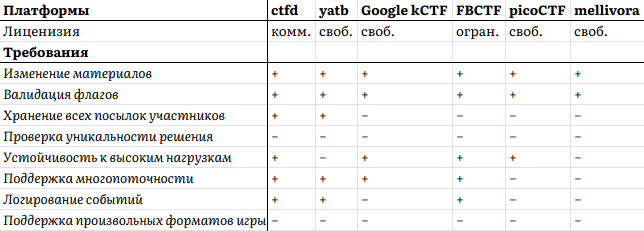
\includegraphics[width=0.9\textwidth]{inc/img/boards-table}\\
  Таблица 2.1. Сравнительный анализ наиболее популярных платформ для Jeopardy CTF
  \label{fig:jeopardy}
\end{figure}

Существует множество программных продуктов, позволяющих проводить jeopardy -- CTF-соревнования: организаторам необходимо лишь собрать участников, разработать задания и загрузить их на готовую платформу.

Анализ наиболее популярных готовых проверяющих систем для Jeopardy CTF показал, что ни одна такая система не удовлетворяет всем необходимым требованям (табл. 2.1). Выборка состоит из трёх систем, наиболее популярных на ресурсе GitHub\cite{GithubCTFTag} по тегу «ctf board» (yatb, picoCTF, mellivora), а также трёх систем, которые используются для проведения наиболее популярных международных соревнований по статистике агрератора CTFTime.org\cite{CTFTime}.

\section{Система, предоставляющая очным участникам программную среду для решения задач}

\subsection{Требования к системе}

\subsubsection{Организационные требования к системе}

Каждому участнику на площадке предоставляется компьютер.

Программная среда компьютера должна быть пригодной для решения CTF-задач: нужен Linux с правами администратора (чтобы устанавливать своё ПО, изменять конфигурацию системы и т.п.).

\subsubsection{Технические требования к системе}

\subsection{Установка и инициализация системы}

Поскольку компьютеры не наши, жёсткий диск лучше не трогать.

Следовательно, среду лучше записывать на внешний загрузочный носитель — причём, участнику давать доступ к виртуальной машине, а в родительской ОС разместить инструменты прокторинга и провизии.

\subsection{Виртуализация среды}

Использование виртуальной машины подразумевает наличие какого-то образа ОС. Поскольку это непринциаильный момент, можно предусмотреть возможность участника, при его желании, использовать свой образ ОС, а также поставлять универсальный «нейтральный» образ любого подходящего дистрибутива ОС Linux. Например, Kali Linux — наиболее распространённый дистрибутив, в комплекте поставки которого содержится большое количество инструментов для исследования уязвимостей.

Таким образом, можно сформулировать требования к функциональности такой системы.

\subsection{Контроль целостности системы}

\subsection{Контроль соблюдения правил олимпиады}

\subsubsection{Прокторинг}

\subsubsection{Захват и анализ содержимого на экране комьютера}

\subsubsection{Захват и анализ сетевого трафика}

\subsection{Провизия системы}

\subsubsection{Предоставление личных сведений об участнике}

\subsubsection{Удалённое управление компьютерами}

\begin{figure}
  \centering
  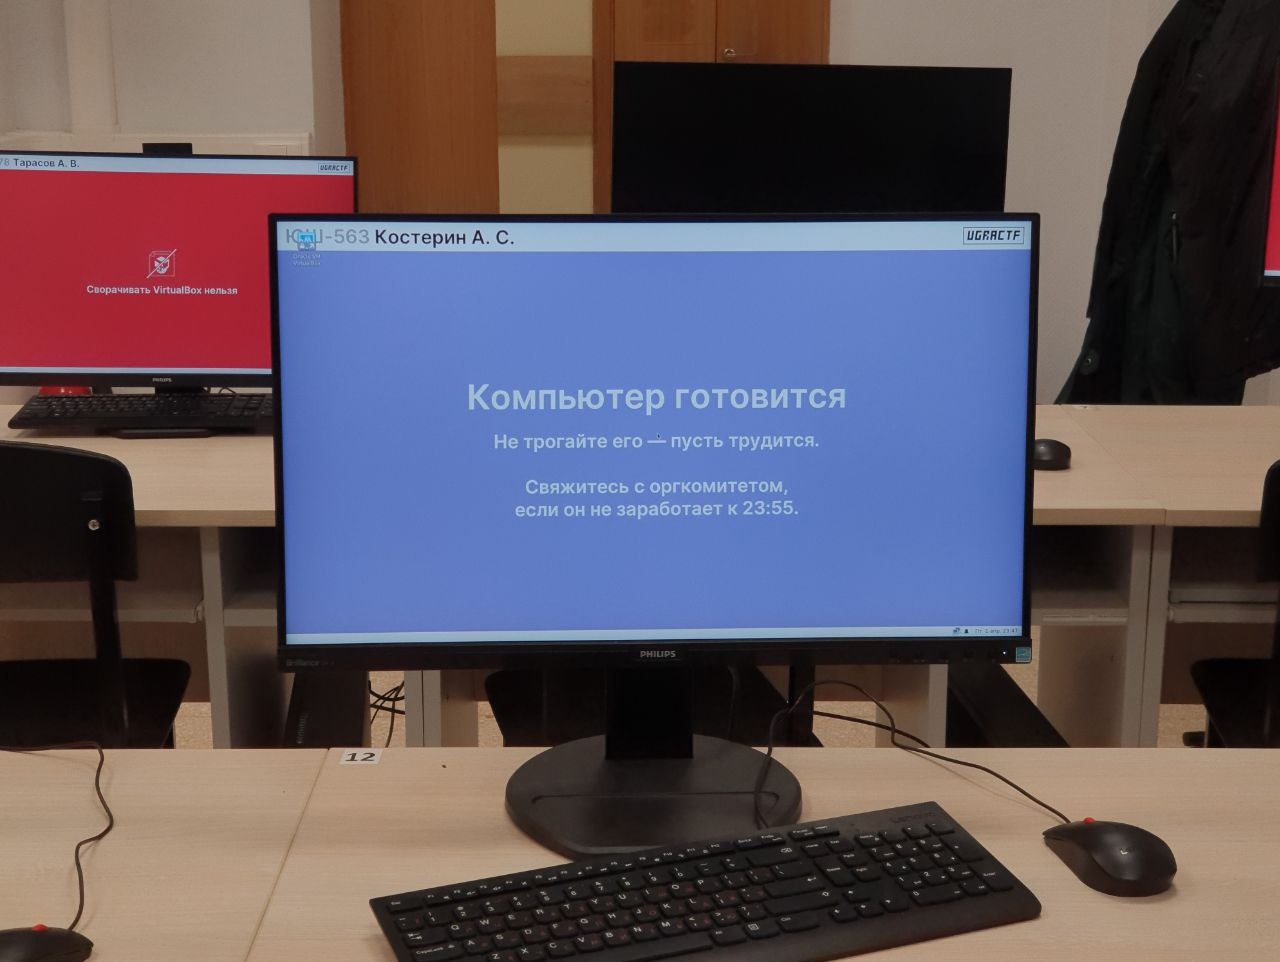
\includegraphics[width=0.7\textwidth]{inc/img/ugra-schoolos}
  \caption{Инициализация системы SchoolOS на соревнованиях Ugra CTF School 2022 в Долгопрудном}
  \label{fig:jeopardy}
\end{figure}

\begin{enumerate}
\item Автоматически разворачивается виртуальная машина с образом ОС, заблаговременно предоставленным участником через свой личный кабинет;
\item Все остальные приложения полностью изолируются от участника;
\item Реализованы элементы прокторинга: периодически с машины каждого участника собираются скриншоты, которые в перспективе планируется автоматически анализировать на предмет нарушения правил — там всё неочевидно, поскольку мы разрешаем пользоваться интернетом, но запрещаем любую внешнюю помощь и распространение условий задач;
\item Настраивается сетевой тоннель в общую игровую сеть;
\item Обеспечивается возможность удалённого доступа организаторов к любой машине;
\item Гарантируется невозможность модификации запущенной хост-ОС: её системных файлов, конфигурации ПО и пользователей с группами.
\end{enumerate}

Прокторинг:
\begin{itemize}
\item
  запись экрана;
\item
  контроль целостности ОС.
\end{itemize}

Провизия:
\begin{itemize}
\item
  участники могут работать в любой ОС, образ которой заблаговременно предоставят, либо в стандартом окружении Kali Linux (вариант по умолчанию);
\item
  конфигурация сети;
\item
  вывод на рабочем столе сведений об участниках («подписать», где чей компьютер);
\item
  возможность удалённого доступа к каждой машине для администрирования.
\end{itemize}




\section{Общая модель системы}

\subsection{Модель компьютерной системы}

\begin{itemize}
\item
  сервер жюри с бордой (веб-интерфейс, HTTPS);
\item
  сервер провизии и прокторинга (управление через SSH);
\item
  хранилище образов ВМ участников;
\item
  рабочие места участников.
\end{itemize}

\section{Модель угроз}

\subsection{Модель нарушителя}

Участник:
\begin{itemize}
\item
  может общаться в интернете
\item
  может обмениваться флагами с другими участниками
\item
  может обмениваться условиями задач с внешним миром
\item
  может атаковать инфраструктуру (в разных местах)
\end{itemize}

Организатор:
\begin{itemize}
\item может помогать участникам
\item может получить доступ к условиям задач
\item может не пресекать нарушения правил
\end{itemize}
